\documentclass[tikz,border=10pt]{standalone}
\begin{document}
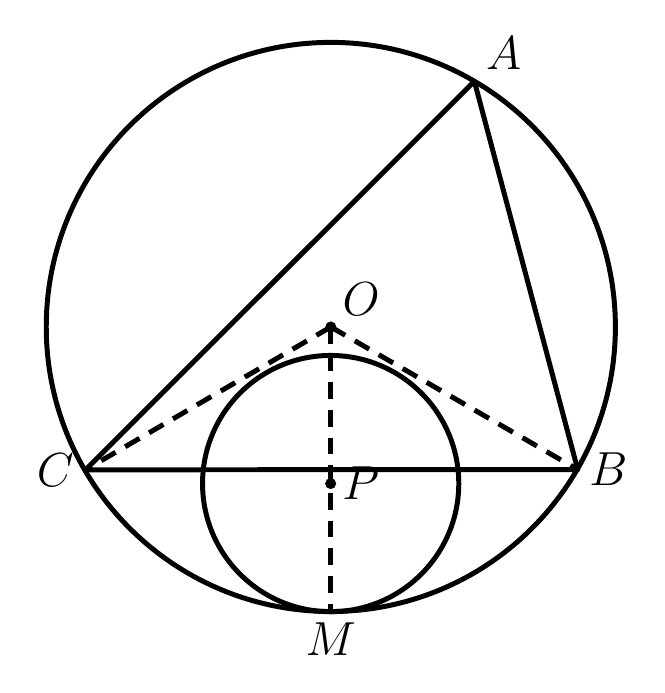
\begin{tikzpicture}[line width=1.8pt, line join=round]
% Scale: s = 0.022989 cm per px, centred on ink bbox centre (203,210) px, y flipped
% Named coordinates
\coordinate (O) at (-0.016,0.253);   % centre of large circle
\coordinate (A) at (1.807,3.373);    % top point on large circle
\coordinate (B) at (3.120,-1.559);   % right point on large circle
\coordinate (C) at (-3.131,-1.561);  % left point on large circle
\coordinate (P) at (-0.018,-1.736);  % centre of small circle
\coordinate (M) at (-0.016,-3.361);  % tangency point (bottom)

% Large circle (radius 3.614) and small circle (radius 1.627), both solid
\draw (O) circle (3.614);
\draw (P) circle (1.627);

% Solid triangle AC, CB, BA
\draw (A) -- (C) -- (B) -- cycle;

% Long-dash style for auxiliary segments OC, OB and vertical OM
\tikzset{longdash/.style={dash pattern=on 6pt off 4pt}}
\draw[longdash] (O) -- (C);
\draw[longdash] (O) -- (B);
\draw[longdash] (O) -- (M);

% Filled dots at O and P (same size)
\fill (O) circle (0.07);
\fill (P) circle (0.07);

% Labels: italic serif math, 16.5 pt font from STYLE METRICS
\node[font=\fontsize{16.5}{19.8}\selectfont, anchor=south west] at (A) {$A$};
\node[font=\fontsize{16.5}{19.8}\selectfont, anchor=south west] at (O) {$O$};
\node[font=\fontsize{16.5}{19.8}\selectfont, anchor=west] at (P) {$P$};
\node[font=\fontsize{16.5}{19.8}\selectfont, anchor=east] at (C) {$C$};
\node[font=\fontsize{16.5}{19.8}\selectfont, anchor=west] at (B) {$B$};
\node[font=\fontsize{16.5}{19.8}\selectfont, anchor=north] at (M) {$M$};
\end{tikzpicture}
\end{document}